\section{Zielsetzung}
\label{sec:ziel}

In diesem Versuch sollen Scanverfahren der Ultraschalltechnik näher untersucht und angewendet werden.

\section{Theorie}
\label{sec:Theorie}

In einem Frequenzbereich von $\SIrange{16}{20}{\kilo\hertz}$ kann ein Mensch hören. Frequenzen oberhalb dieser Hörschwelle, etwa in einem Bereich von $\SI{20}{\kilo\hertz}$ 
bis $\SI{1}{\giga\hertz}$, werden \textit{Ultraschall} genannt. Unterhalb dieser Grenze wird von \textit{Infraschall} gesprochen. Die Frequenzen oberhalb des Frequenzbereiches des Ultraschalls 
werden als \textit{Hyperschall} bezeichnet. 
Ultraschall wird mithilfe des \textit{piezo-elektrischen Effektes} erzeugt. Ein piezoelektrischer Kristall wird dabei in einem elektrischen Wechselfeld so angeregt, dass er Ultraschall emittiert. Das Konzept
kann auch umgekehrt genutzt werden, sodass ein piezoelektrischer Kristall als Empfänger für Ultraschall verwendet wird. \newline
Schall ist eine longitudinale Welle, die sich durch Druckschwankungen ausbreitet und mit der folgenden Gleichung beschrieben werden kann,
\begin{align}
    \label{eqn:druckgleichung}
    p(x,t)=p_0+v_0Z\cos\left(\omega t-kx\right).
\end{align}
Dabei steht $Z$ für die \textit{akustische Impedanz} und kann durch die Dichte $\rho$ des durchschrittenen Mediums und der Schallgeschwindigkeit in diesem Material $\nu$
mit $Z=\rho\cdot\nu$ beschrieben werden. Wie jede Welle auch, weist eine Schallwelle Reflexions- und Beugungseigenschaften auf. Die Phasengeschwindigkeit einer Schallwelle ist allerdings materialabhängig.
In Gasen und Flüssigkeiten breitet sich eine Schallwelle immer als Longitudinalwelle aus und die Schallgeschwindigkeit in einer Flüssigkeit ist von ihrer \textit{Kompressibilität} $\kappa$
und ihrer Dichte $\rho$ abhängig,
\begin{align}
    \label{eqn:SchallFlüssig}
    \nu_{\text{Fl}} = \sqrt{\frac{1}{\kappa\cdot\rho}}.
\end{align}
In einem Festkörper dagegen breitet sich Schall infolge von Schubspannungen nicht nur als Longitudinalwelle, sondern auch als Transversalwelle aus. Die Schallgeschwindigkeit in einem Festkörper folgt zu,
\begin{align}
    \label{eqn:SchallFest}
    \nu_{\text{Fe}} = \sqrt{\frac E\rho},
\end{align}
wobei $E$ das Elastizitätsmodul ist. Da bei der Schallausbreitung ein Teil der Energie in Form von Absorptionsprozessen verloren geht, nimmmt die Intensität mit zunehmend zurückgelegter Entfernung $x$ exponentiell ab,
\begin{align}
    \label{eqn:intensitaetsverlust}
    I(x)=I_0\cdot e^{\alpha ~ x}.
\end{align}
Dabei ist $\alpha$ der materialabhängige Absorptionskoeffizient der Schallamplitude. \newline
Schall wird in Luft sehr stark gedämpft, weshalb zwischen dem Schallgeber und dem zu untersuchenden Material häufig ein Kontaktmittel verwendet wird. Wenn eine Schallwelle auf eine Grenzfläche, zum Beispiel das Kontaktmittel, trifft, so wird
ein Teil der Schallwelle reflektiert. Der Reflexionskoeffizient $R$ wird dabei aus dem Verhältnis von reflektierter und einfallender Schallintensität gewonnen und lautet bei angrenzenden Materialien
\begin{align}
    \label{eqn:Reflexionskoeffizient}
    R=\left(\frac{Z_1-Z_2}{Z_1+Z_2}\right)^2.
\end{align}
Der Transmittierte Anteil $T$ lässt sich mit $T=1-R$ bestimmen. \newline
Bei Ultraschallmessungen werden im Allgemeinen zwei verschiedenen Verfahren unterschieden. Das \textit{Durchschallungs-Verfahren} und das \textit{Impuls-Echo-Verfahren}.

\subsection*{Durchschallungs-Verfahren}
\label{subsec:durchschallungVerfahren}
Beim Durchschallungs-Verfahren wird mit einem Ultraschallsender ein kurzzeitiger Impuls ausgesendet und mit einem Ultraschallempfänger am anderen Ende der Messprobe detektiert.
Befindet sich in der Probe eine dichtere Stelle, also eine Fehlstelle, dann wird eine abgeschwächte Intensität am Empfänger gemessen. Bei einem Loch in der Probe ist zwar die Fehlstelle nicht dichter, die Dämpfung in Luft
ist aber höher, sodass auch hier eine Abgeschwächte Intensität gemessen wird. Eine Aussage über die Position der Fehlstelle kann nicht getroffen werden.
In \autoref{fig:durchschallung} ist eine schematische Darstellung des Verfahrens und des \textit{Laufzeitdiagrammes} einer Messung mit der Durchschallungs-Methode abgebildet.

\begin{figure}[H]
    \centering
    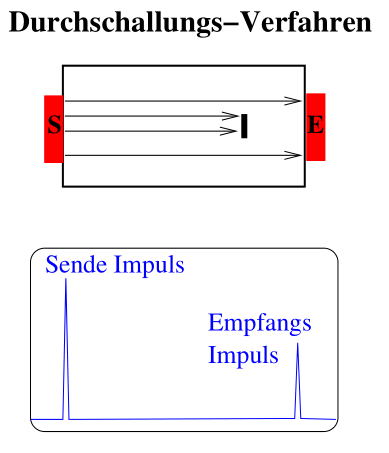
\includegraphics[width=0.3\textwidth]{data/Durchschallungsverfahren.png}
    \caption{Schematische Darstellung des Durchschallungsverfahren \cite{AnleitungUS2}.}
    \label{fig:durchschallung}
\end{figure}

\subsection*{Impuls-Echo-Verfahren}
\label{subsec:ImpEcho}

Beim Impuls-Echo-Verfahren wird der Ultraschallsender auch als Empfänger verwendet. Der ausgesendete Ultraschallimpuls wird an einer Grenzfläche reflektiert und wieder am Empfänger detektiert. Durch die Laufzeit des
Ultraschalls kann bei der Impuls-Echo-Methode eine Aussage über die Position der Fehlstelle getroffen werden. Bei bekannter Schallgeschwindigkeit wird die Lage der Fehlstelle durch die Gleichung 
\begin{align}
    \label{eqn:lageFehler}
    s = \frac 12 v t
\end{align}
bestimmt. 
In \autoref{fig:durchschallung} ist eine schematische Darstellung des Verfahrens und des Laufzeitdiagrammes einer Messung mit der Impuls-Echo-Methode abgebildet.
\begin{figure}[H]
    \centering
    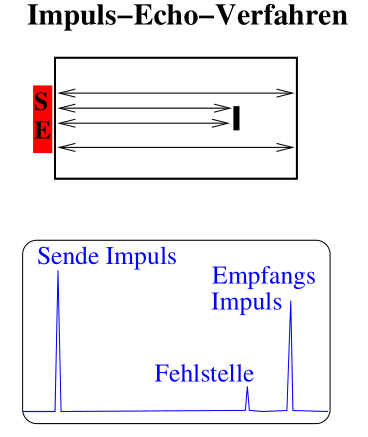
\includegraphics[width=0.3\textwidth]{data/ImpulsEchoVerfahren.png}
    \caption{Schematische Darstellung des Impuls-Echo-Verfahrens \cite{AnleitungUS2}.}
    \label{fig:impulsEcho}
\end{figure}
Laufzeitdiagramme werden in verschiedenen Darstellungsarten für verschiedene Anwendungszwecke etstellt.
\begin{enumerate}
    \item Der \textit{Amplituden-Scan} (A-Scan) ist ein eindimensionales Verfahren zur Abtastung von Strukturen. Es wird die Amplitude gegen die Laufzeit dargestellt.
    \item Der \textit{Brightness-Scan} (B-Scan) ist ein zweidimensionales Verfahren, bei dem durch Bewegen der Sonde ein Bild aus Helligkeitsabstufungen erstellt wird.
    \item Der \textit{Time-Motion-Scan} (TM-Scan) erstellt durch schnelle Abtastung eine zeitliche Bildfolge, um zum Beispiel die Bewegungen eines Organes sichtbar zu machen.
\end{enumerate}
